\pagebreak
\subsection{Electrical Design}

\subsubsection{Block Diagrams}
\begin{centering}
The electronics design can be seen in Figure \ref{fig:electronics-block-diagram} and the interfaces this requires can be seen in Figure \ref{fig:eee-interface-diagram}. There will be four distinct areas, the Electronics box, the valve centre, the pump box and the CAC system. All connections to the outside of the box are located in the electronics box. These are the voltage regulators for the external power source and the Ethernet shield with an SD data storage which will connect to the Telemetry, Tracking, and Command (TT\&C). Additionally one pressure sensor, one heater and one temperature sensor will be placed in this area. The CAC system area will contain three temperature sensors to monitor its ambient temperature and one electronic valve to be closed before landing. In the AAC system area there will be eleven valves, one airflow sensor, one pressure sensor, five temperature and one humidity sensor and a heater. In the pump box there will be the miniature diaphragm air pump, one temperature sensor and one heater.
\end{centering}
\bigskip

\begin{figure}[H]
    \begin{align*}
        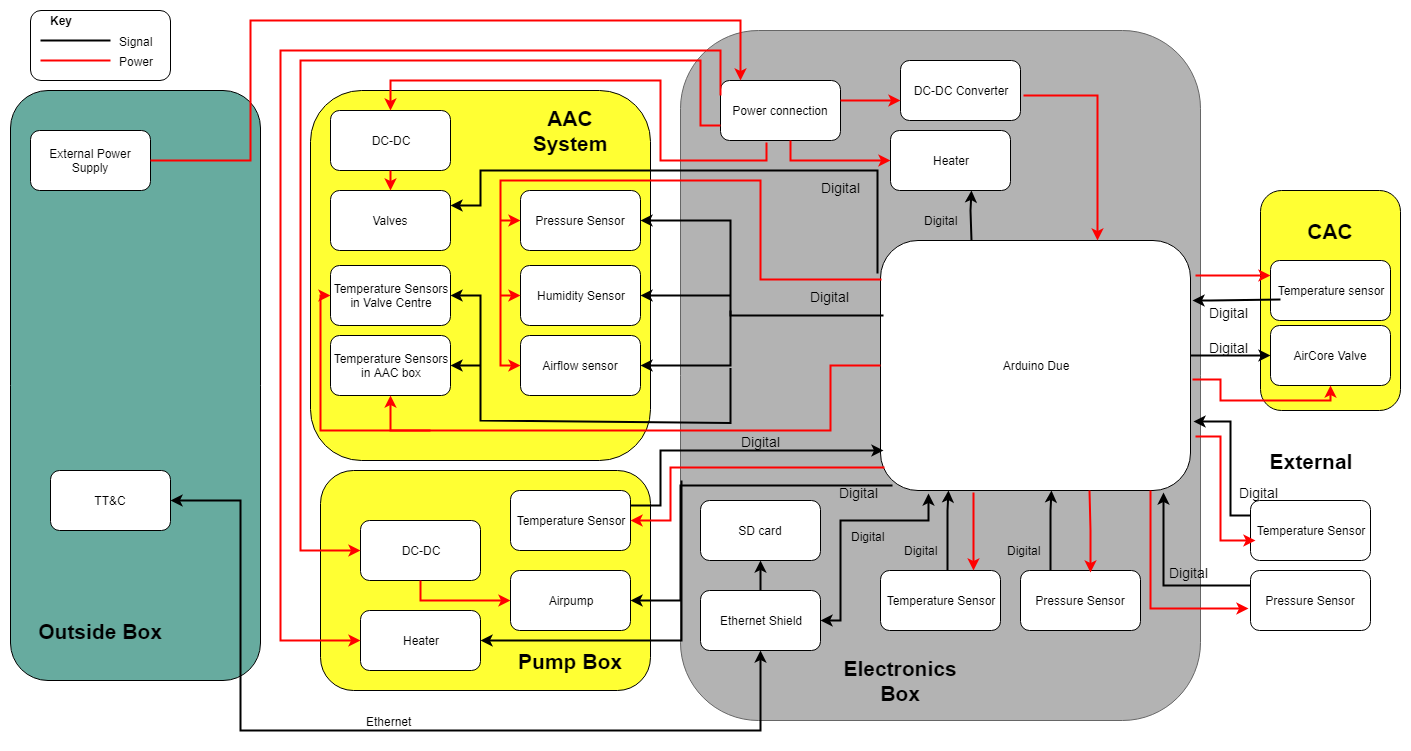
\includegraphics[width=16cm]{4-experiment-design/img/block-diagram-four-sections.png}
    \end{align*}
    \caption{Block Diagram for all Electronic Components Showing the Signal and Power Connections}\label{fig:electronics-block-diagram}
\end{figure}


\begin{figure}[H]
    \begin{align*}
        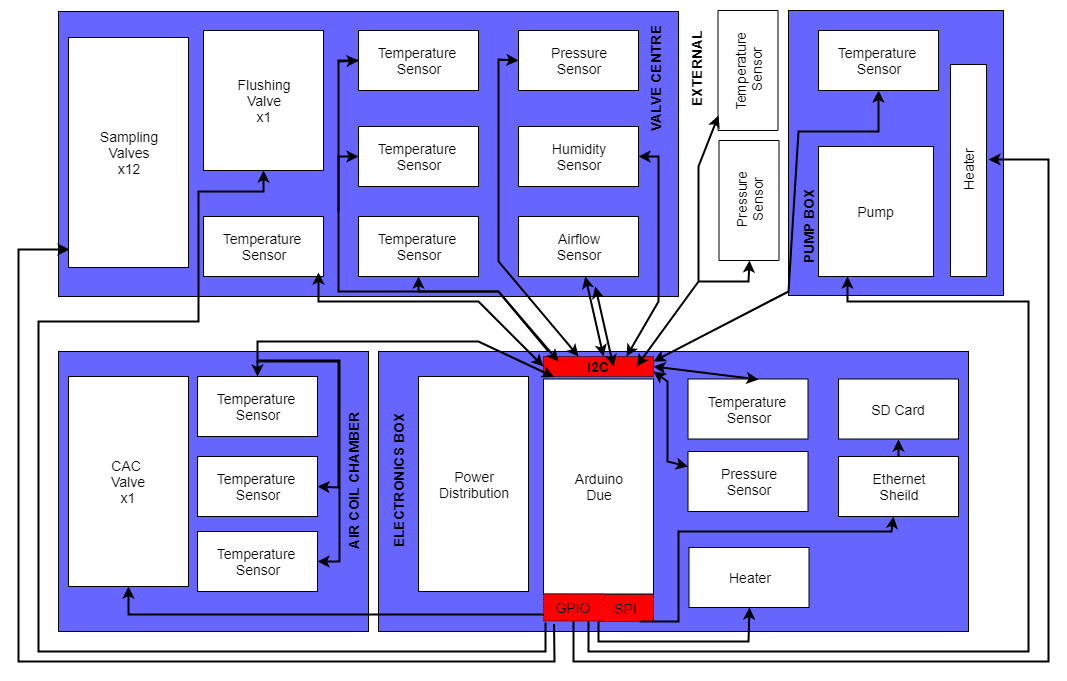
\includegraphics[width=16cm]{4-experiment-design/img/INTERFACE-DIAGRAM-2.png}
    \end{align*}
    \caption{Block Diagram Showing the Interfaces Between All Electrical Components.}\label{fig:eee-interface-diagram}
\end{figure}

\begin{centering}
Three DC-DC converters will be used to step down the voltage from the 28.8V provided by the gondola down to: 
\end{centering}

\begin{centering}
\begin{itemize}
  \item $28.8V \Longrightarrow 12V$ for the Arduino.  
  \item $28.8V \Longrightarrow 24V$ for the valves.
  \item $28.8V \Longrightarrow 24V$ for the pump.
  \end{itemize}

\end{centering}
\bigskip

\begin{centering}
The heaters will not require the voltage to be stepped down and so will be powered directly from the gondola battery.
\end{centering}
\bigskip

\subsubsection{Miniature Diaphragm Pump}
The pump which has been selected is the KNF 850.1.2. KNDC B, Figure \ref{fig:pumppic}, which is manufactured by KNF. One of the reasons this pump has been selected is that it has successfully been flown on a similar flight in the past \cite{LISA}. On this flight it managed to pump 180mL of air at 25km altitude. However, to ensure the pump will operate as intended several low pressure and low temperature tests will be completed.

The pump has a maximum flow rate of 8.0LPM when at ambient pressure. This is in excess of the required flow rate as the flow rate will decrease as the altitude increases. As the pressure decreases the current required by the pump will increase until it hits a peak current draw of 340mA. However as seen in Figure \ref{fig:pumpflowcur} the peak current then decreases as the pressure continues to decrease. It is also worth noting that whilst the flow rate appears to decrease too much Figure \ref{fig:pumpflowcur} is assuming that this is the pressure differential. Our bags will not be at vacuum and they will not be pressurized therefore the expected flow rate performance is higher.

\begin{figure}[H]
    \begin{align*}
        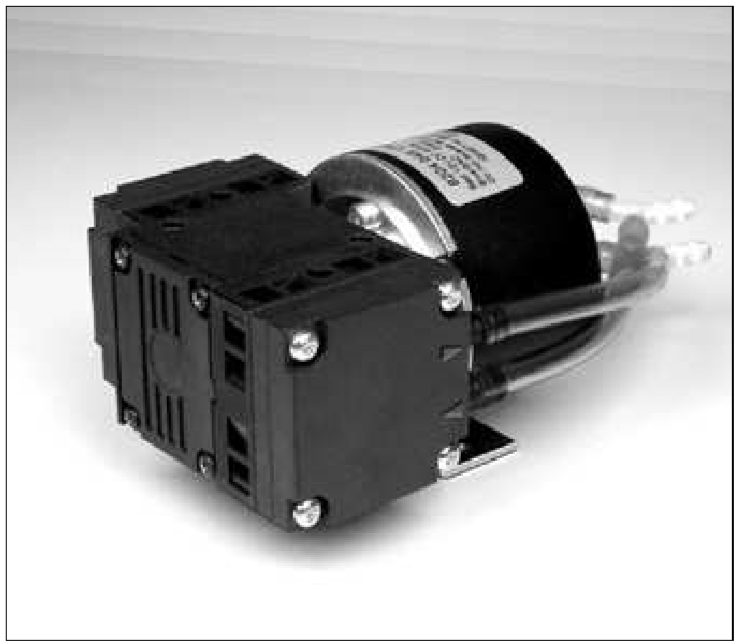
\includegraphics[width=6cm]{4-experiment-design/img/pump-850-1-2-kndc-b.png}
    \end{align*}
    \caption{KNF 850.1.2. KNDC B Miniature Diaphragm Pump}\label{fig:pumppic}
\end{figure}


\begin{figure}[H]
    \begin{align*}
        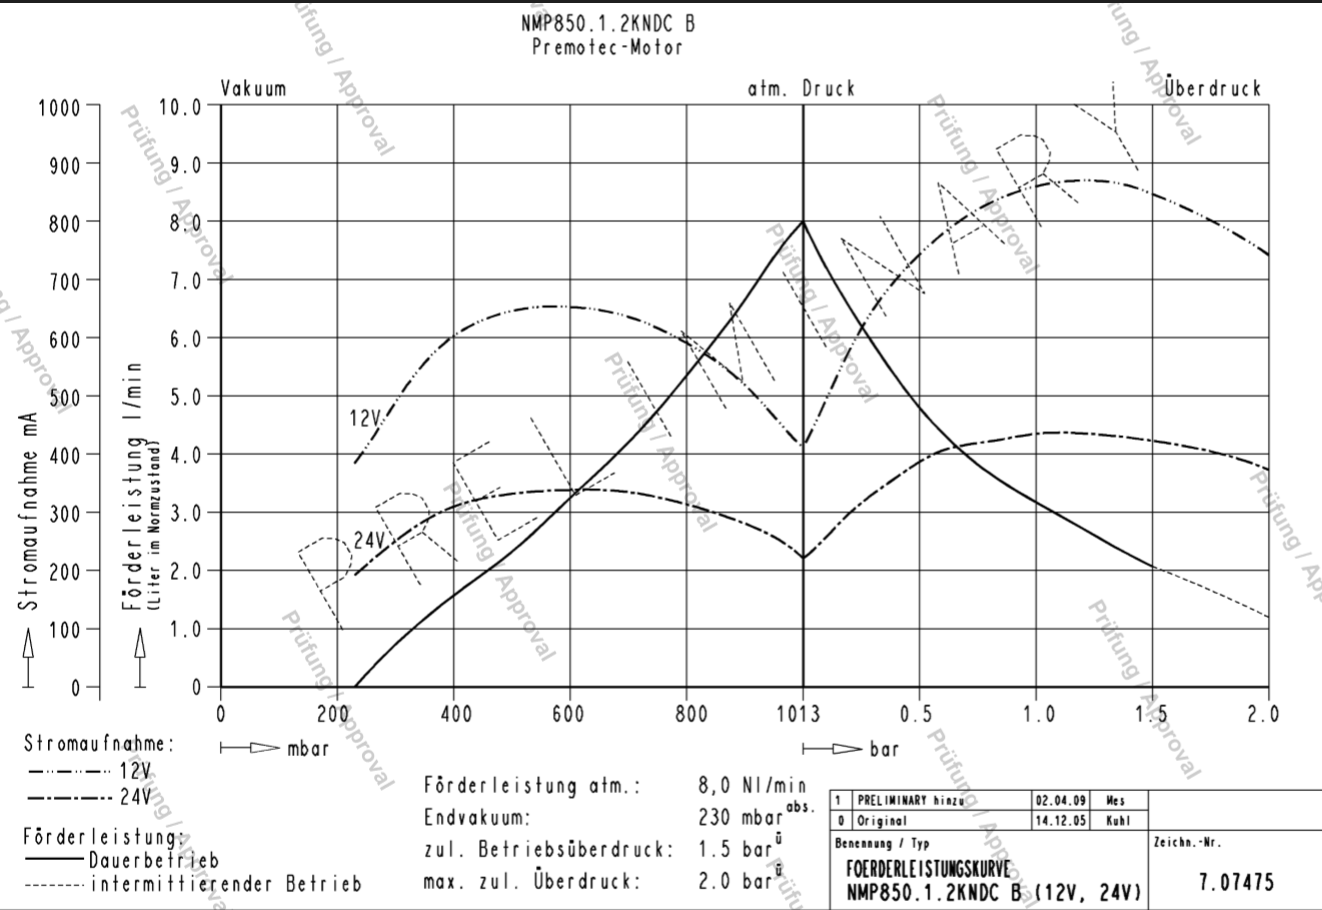
\includegraphics[width=15cm]{4-experiment-design/img/pump-flow-rate-current-graph.png}
    \end{align*}
    \caption{KNF 850.1.2. KNDC B Flow Rate and Current Draw to Pressure Graph.}\label{fig:pumpflowcur}
\end{figure}


\subsubsection{Electromagnetically Controlled Valves}
Filling of the air bags will be controlled by the solenoid valves. For this purpose Parker solenoid valve 121K63, Figure \ref{fig:valve},  with the 24 VDC coil, Figure \ref{fig:coil}, has been selected after careful consideration of the different options available in the market and keeping the experiment requirements in mind. The valves will be normally closed through out the experiment with zero power consumption and will be open, when given power, to fill up the air bags at specific altitudes or to flush the tubes.

\begin{figure}[H]
    \begin{align*}
        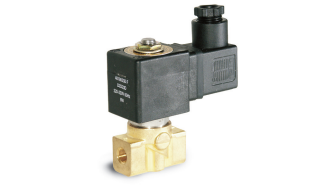
\includegraphics[width=6cm]{4-experiment-design/img/valve.png}
    \end{align*}
    \caption{Valve}\label{fig:valve}
\end{figure}

\begin{figure}[H]
    \begin{align*}
        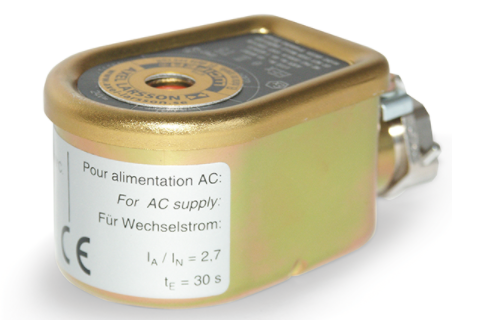
\includegraphics[width=2cm]{4-experiment-design/img/Coil.png}
    \end{align*}
    \caption{Coil}\label{fig:coil}
\end{figure}


The port size of the valve is 1/4" which is compatible with the gas analyzer. The coil can withstand temperature from -40 to 50 °C which is suitable for flight operations at high altitudes. Although the valve can operate under a maximum pressure drop of 100 bar it also needs to be tested at intended low pressure values. For this purpose one valve with the motor and a shield, Figure \ref{fig:shield}, has already been ordered.  


\begin{figure}[H]
    \begin{align*}
        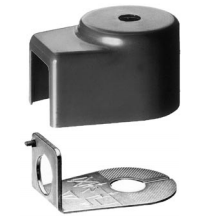
\includegraphics[width=2cm]{4-experiment-design/img/Shield.png}
    \end{align*}
    \caption{Shield}\label{fig:shield}
\end{figure}

\subsubsection{Valve Driving Circuit}
The valves will be powered through a 50W DC-DC converter that will step down the 28.8V to 24V. They will also have a connection to the Arduino so that they can be controlled. In order to allow this connection a switching circuit has been devised using a power MOSFET and a BJT. This circuit is detailed in Figure \ref{fig:switchcir}.

\begin{figure}[H]
    \begin{align*}
        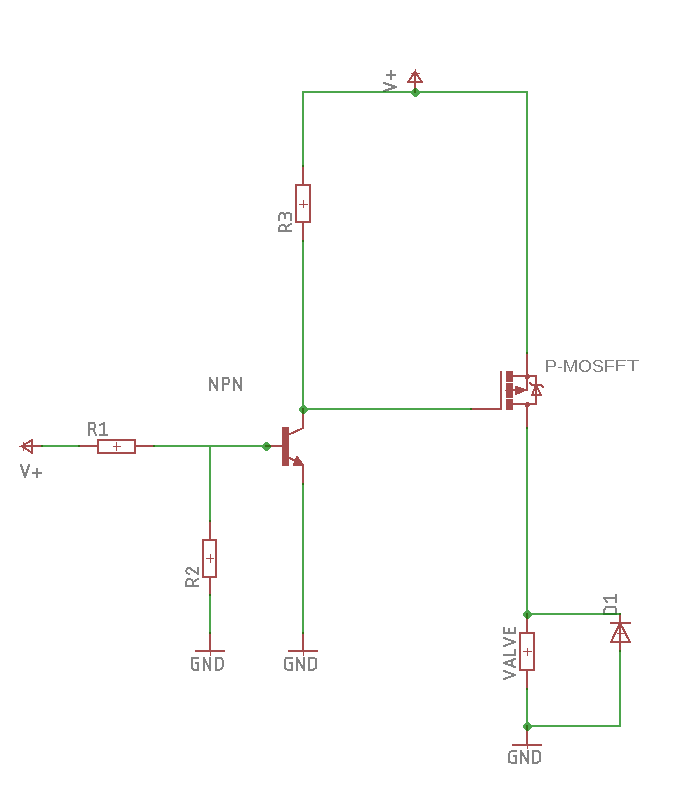
\includegraphics[width=8cm]{4-experiment-design/img/switching-circuit-2.png}
    \end{align*}
    \caption{Schematic showing the switching circuit to drive the valves through the Arduino}\label{fig:switchcir}
\end{figure}

The power MOSFET will control the valves ON-OFF state whilst the BJT will connect directly to the Arduino and ensure that the valve is only turned on when a true signal is given. The power MOSFET will be on when the BJT is on. The BJT will be on when a signal of 3.3V is given and off when a signal of 0V is given. Three resistors will also be used. The purpose of $R_{1}$ is to protect the Arudino and also to step up the current entering the BJT. The value has been chosen to ensure that enough current reaches the valve to turn it on. $R_{2}$ is an optional resistor which creates a voltage divider that further increases the current entering the BJT. Finally $R_{3}$ is for when the BJT is off to avoid creating a short circuit. 


\raggedbottom